\chapter{Results}\label{chap:results}

Chapter \ref{chap:methods} built three solvers. The LM solver, the NN solver, and the hybrid solver. This chapter evaluates each of the three solvers on a held-out test set and compares them against one another. 

The chapter contains three steps. Section \ref{sec:results-lm} measures how good an initialisation must be for LM to converge, Section \ref{sec:res-network} measures how good the network's predictions are, and Section \ref{sec:three_way} tests whether the network initialisation is good enough for the LM solver to converge. We close the chapter by discussing the implications of these results.

\section{Experimental Setup}
All models are evaluated on the same held out test set consisting of $N_{\mathrm{test}}$ datapoints, generated separately from the training/validation datapoints. The data splits are shown in Table \ref{tab:data_splits}.  


\subsection{Hardware Setup}
Training and inference times are reported throughout this chapter. All computation is done on the same machine with specifications shown in Table \ref{tab:comp_specs}. Models are trained purely on the CPU. In reporting we use the CPU time, not the wall time, because some processes are singlethreaded whereas others are multithreaded. For example, NN training is multi-threaded, whereas LM inference is single-threaded. 

\begin{table}
  \centering
  \begin{tabular}{ll}
    \toprule
    Component & Model \\
    \midrule
    CPU  & AMD Ryzen 5 1600x \\
    RAM  & 32GB DDR4 2133MT/S \\
    \bottomrule
  \end{tabular}
  \caption{Computer specifications for training and inference}
  \label{tab:comp_specs}
\end{table}

\subsection{Convergence Criteria}\label{sec:conv_criteria}
In Section \ref{sec:methods-lm} we define two constants, $\epsilon_p$ and $\epsilon_n$, which dictate when we consider a run to have \emph{converged}. In this chapter, we use the values shown in Table \ref{tab:conv_criteria}. A solve is said to have converged if the positional and angular errors are both less than $\epsilon_p$ and $\epsilon_n$, respectively.

\begin{table}
  \centering
  \begin{tabular}{ll}
    \toprule
    Parameter & Value \\
    \midrule
    $\epsilon_p$  & 1\,mm \\
    $\epsilon_n$ & 1$^\circ$ \\
    \bottomrule
  \end{tabular}
  \caption{Convergence criteria for results reporting.}
  \label{tab:conv_criteria}
\end{table}

\section{The Levenberg-Marquardt Solver}\label{sec:results-lm}
Section \ref{sec:methods-lm} shows how we implement the LM solver. This section shows its performance and motivates the need for NN initialisation.

\subsection{Basin Sweep}
We want to know how accurate an initialisation must be before LM can recover the pose. We therefore work out how "bad" an initialisation can be to give a desired convergence rate. 
\paragraph{Method -} $N_{\mathrm{bs}} = 200$ poses are sampled from the held-out test set with a fixed seed. We then perform two independent perturbation sweeps: A positional sweep and an angular sweep. The position perturbation is generated by picking a random direction via Gaussian sampling. Then normalising that vector and multiplying by the perturbation distance, $d$. The angular perturbation requires some consideration. 

If we want to perturb an orientation vector $\hat{n} = (n_1,n_2,n_3)$ by an angle $\alpha$, we generate a random vector from a Gaussian distribution $v \sim \mathcal{N}(0,I_3)$. Then we project $v$ onto the plane perpendicular to $\hat{n}$, as in equation \eqref{eq:proj_v_n}. After this, we normalise $v_{\perp}$ and rotate by $\alpha$ in the direction of $v_{\perp}$ as in equation \eqref{eq:rotation}.

\begin{equation}
  v_{\perp} = v - (v \cdot \hat{n}) \hat{n}
  \label{eq:proj_v_n}
\end{equation}

\begin{equation}
  \hat{n}_\mathrm{pert} = \cos(\alpha) \hat{n} + \sin(\alpha) (v_{\perp} / \left\vert v_{\perp} \right \vert)
  \label{eq:rotation}
\end{equation}


For each of the sweeps, the convergence rate is calculated as in Section \ref{sec:conv_criteria}.

\paragraph{Positional Sweep -} The position is swept from $d = 0$ to $d = 150$mm. Figure \ref{fig:pos_sweep} shows that as the perturbation magnitude increases, there is a steady decrease in the convergence rate, with no sharp dropoff. This suggests that there are no sharp boundaries contrary to what one might expect of a Newton-type method. 
\begin{figure}
  \centering 
  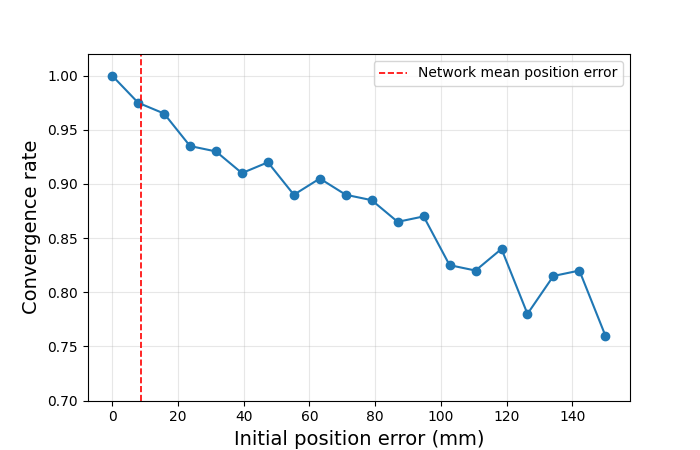
\includegraphics[width = 0.8 \textwidth]{figs/pos_sweep.png}
  \caption{Convergence rate against positional perturbation. The dashed line marks the mean positional error of the trained NN seen in Section \ref{sec:res-network}.}
  \label{fig:pos_sweep}
\end{figure}

\paragraph{Angular Sweep -} The angle is swept from $\alpha = 0$ to $\alpha = 90^{\circ}$. Figure \ref{fig:angle_sweep} shows the same story as the positional sweep, steady decrease with no sharp dropoff. We do note that the angle is a lot more forgiving than position, retaining a 97.5\% convergence rate up to $\alpha = 42.6^\circ$. This is because the equation \eqref{eq:forward} depends on $1/r^{3}$ whereas the orientation angle only enters through the dot product.

\begin{figure}
  \centering
  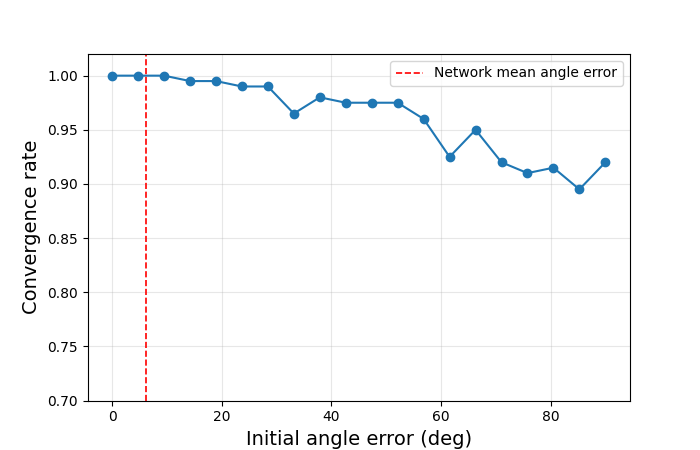
\includegraphics[width = 0.8\textwidth]{figs/angle_sweep.png}
  \caption{Convergence rate against angular perturbation. The dashed line marks the mean angular error of the trained NN.}
  \label{fig:angle_sweep}
\end{figure}

What is interesting in both the positional and angular sweeps is that the failure is discrete. Either the solver converges to machine precision $\sim 10^{-14} \mathrm{mm/}^\circ$ or else it is off by a large number. This is seen when comparing the mean, median, and 95\% error. For example, in the positional perturbation with $d = 86.8$ mm we get a mean positional error of 8.13mm but a median positional error of $1.8*10^{-11}$mm, suggesting that a few outliers inflate the mean. This is further confirmed by the 95\% error of 56.3mm, showing that either the solver works or it does not, there is no slow dropoff in error. This is also shown in Figure \ref{fig:pos_sweep_errors}.


\begin{figure}
  \centering 
  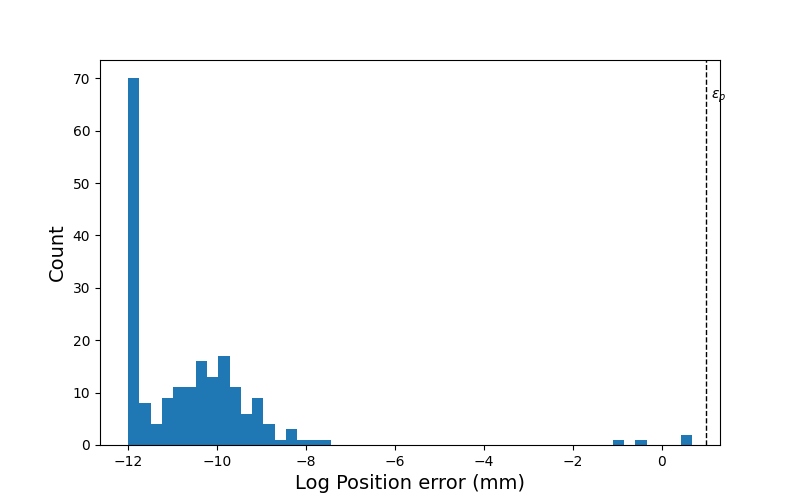
\includegraphics[width = 0.8\textwidth]{figs/pos_sweep_errors.png}
  \caption{Histogram of log positional error for $d = 47.4$mm showing two error classes, failure and convergence.}
  \label{fig:pos_sweep_errors}
\end{figure}

\section{Network Training}\label{sec:res-network}
\subsection{Training Configuration}
In training the network, a number of tuning choices were made against the validation set. First, and most importantly, the network uses the 6-dimensional $(x,y,z,n_1,n_2,n_3)$ pose representation rather than the 5-dimensional $(x,y,z,\theta,\phi)$ representation. Secondly the "PoseLoss" loss function described in Section \ref{sec:methods-loss} was used, instead of MSE. Third, the learning rate was varied using a cosine annealing scheduler, as described in section \ref{sec:network}. Each of these training configurations are shown in  Table \ref{tab:training_config} 
\begin{table}
  \centering
  \begin{tabular}{llllll}
    \toprule
    Name & Target & Loss & LR Scheduler & Optimiser & Epochs\\
    \midrule
    Base & $(\theta,\phi)$ & MSE & None & Adam & 200  \\
    Normal & $\hat{n}$ & MSE & None & Adam & 200\\
    PoseLoss & $\hat{n}$ & PoseLoss & None & Adam & 200 \\
    Final & $\hat{n}$ & PoseLoss & Cosine & Adam & 200 \\
    \bottomrule
  \end{tabular}
  \caption{Experimental Design of NN models.}
  \label{tab:training_config}
\end{table}
\begin{table}
  \centering
  \begin{tabular}{lll}
    \toprule
    Name & Mean Pos Error (mm) & Mean Angular Error (deg)  \\
    \midrule
    Random Pair & 165 & 90 \\
    Centre Predictor & 120 & 90 \\
    Base & 135 & 87.1  \\
    Normal & 139 & 47.7 \\
    PoseLoss & 21.3 & 8.67 \\
    Final & 9.2 & 6.43 \\
    \bottomrule
  \end{tabular}
  \caption{Test set performance of NN models.}
  \label{tab:nn_results}
\end{table}

\paragraph{Base -}Table \ref{tab:nn_results} shows that the base model performs only marginally better than a baseline estimator i.e. it is not much better than a random guess. The expected positional and angular error for two randomly sampled points were estimated using a Monte Carlo simulation drawing from the test set. More interestingly, the base model actually performs worse on position than just guessing the centre of the box every time. This tells us that the base model learns nothing about the orientation and almost nothing about the position.


\paragraph{Normal -}The "Normal" configuration improves the angular error to about half of baseline but left the positional error the same, suggesting that the change to normal parametrisation allows the network to start learning the orientation configuration of the system.

\paragraph{PoseLoss -}The biggest change happens when we change the loss function from MSE to our PoseLoss, reducing positional error by a factor of $6.5$ and angular error by a factor of $5.5$. This change allows the network to actually learn against angular error and also weights the positional and angular error more equally.

\paragraph{Final -}Further refinement is achieved through the use of Cosine learning rate scheduling, allowing training to slow down towards the end, learning the finer details of the data. 
\subsection{Final Model}
The Final NN model, with configuration seen in Table \ref{tab:training_config} was chosen to be used. The number of epochs was chosen to be 200 because by 200 the error on the validation set started plateauing. This plateau can be seen in Figure \ref{fig:training_curves}. 

\begin{figure}
  \centering 
  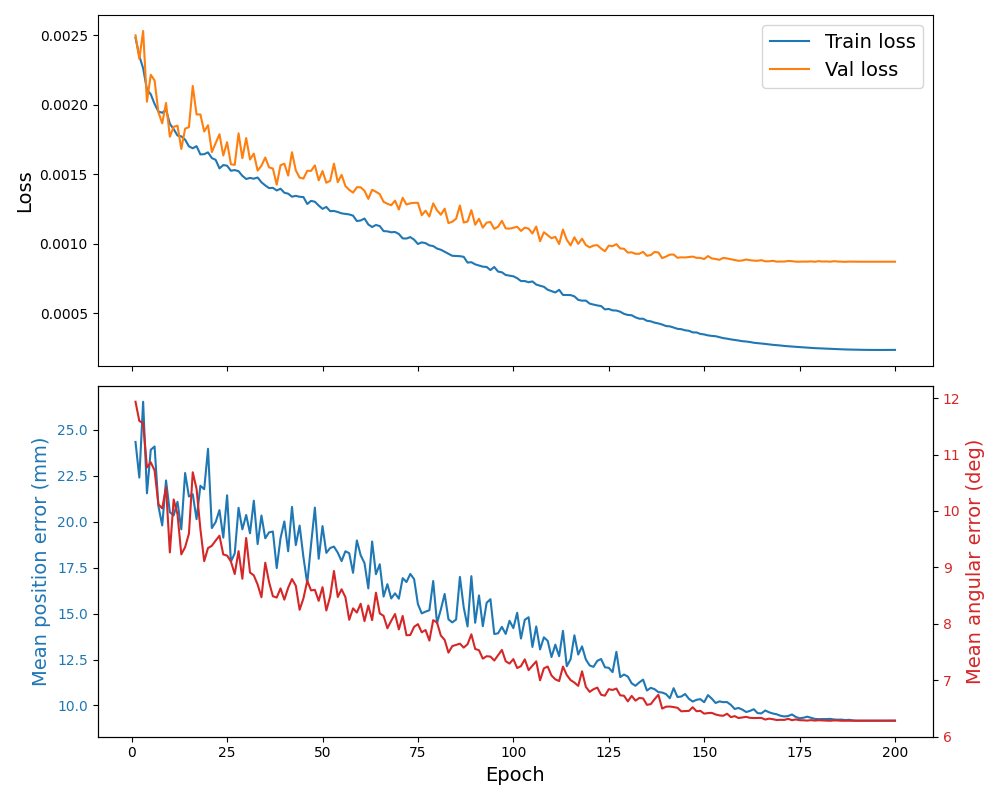
\includegraphics[width = 0.8\textwidth]{figs/training_curves.png}
  \caption{Loss curves and error curves on the validation set}
  \label{fig:training_curves}
 \end{figure}

 \section{Three-way Comparison}\label{sec:three_way}

All three solvers are evaluated on the same held-out test set of 20,000 datapoints. The LM solver uses the same parameters as in section \ref{sec:methods-lm}. The LM model is initialised from the centre of the box with the orientation in the $\hat{z}$ direction. The hybrid solver uses the same solver parameters and differs only in where it starts. The hybrid solver uses the output of the NN as a start point. The results of this test are shown in Table \ref{tab:three_way}. 


\begin{table}
  \centering
  \begin{tabular}{lrrr}
    \toprule
    & LM (cold start) & Network & Hybrid \\
    \midrule
    Mean position error (mm)        & 9.71 & 9.20 & 1.12 \\
    Median position error (mm)      & $1.5\times10^{-11}$ & 7.33 & $3.8\times10^{-12}$ \\
    95th pct.\ position error (mm)  & 64.2 & 21.7 & 1.67 \\
    \addlinespace
    Mean angular error ($^\circ$)       & 8.95 & 6.43 & 1.89 \\
    Median angular error ($^\circ$)     & $5.3\times10^{-12}$ & 3.62 & $1.2\times10^{-12}$ \\
    95th pct.\ angular error ($^\circ$) & 79.5 & 20.9 & 2.46 \\
    \addlinespace
    Convergence rate & 0.859 & 0.0008 & 0.947 \\
    Training time    & --- & 2h 32m 49s & --- \\
    Inference time   & 16m 3s & 361\,ms & 5m 45s \\
    \bottomrule
  \end{tabular}
  \caption{Performance of the three solvers on the held-out test set of
  20{,}000 poses.}
  \label{tab:three_way}
\end{table}

The LM and NN solvers obtain similar mean positional errors, however these solvers operate very differently. The LM solver is extremely bimodal, it either converges to a tiny error on the order of $10^{-11}$mm or else it completely fails. This behaviour is seen when we look at the median and 95th percentile position errors. The NN, on the other hand, has a unimodal distribution of positional errors, with mean, median, and 95th percentile error on similar scales. This suggests that NN performs similarly on almost all poses. This behaviour is seen in Figures \ref{fig:three_way_pos} and \ref{fig:three_way_angle}.

\begin{figure}
  \centering 
  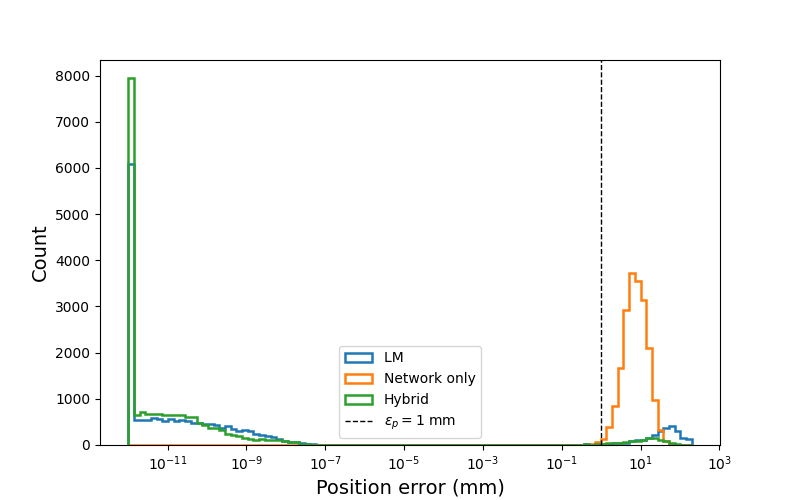
\includegraphics[width=0.8\textwidth]{figs/three_way_pos.png}
  \caption{Histogram of positional errors for each of the three solvers.}
  \label{fig:three_way_pos}
\end{figure}

\begin{figure}
  \centering 
  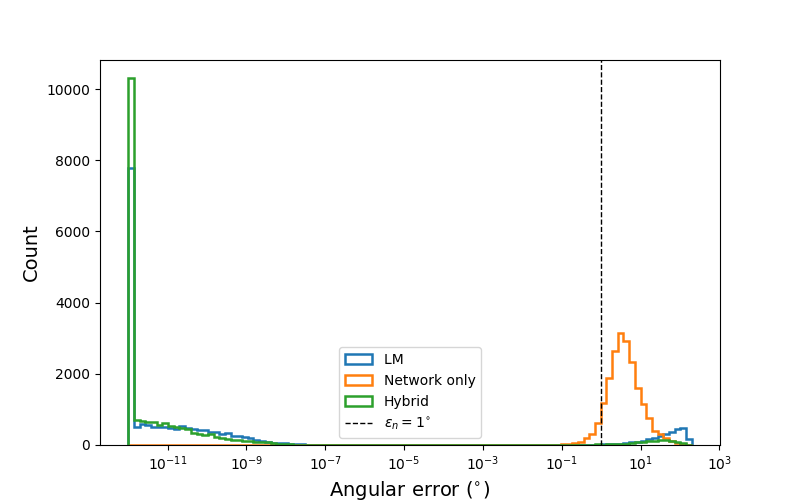
\includegraphics[width = 0.8\textwidth]{figs/three_way_angle.png}
  \caption{Histogram of angular errors for each of the three solvers.}
  \label{fig:three_way_angle}
\end{figure}

The goal of the Hybrid solver is to push the LM into the low error mode. We see in Table \ref{tab:three_way} that it succeeds in this goal. It decreases the rate of non-convergence by a factor of $2.66$. The median errors of the Hybrid solver remain similar to that of the LM solver, however the mean and 95th percentile errors decrease drastically. Looking at the rightmost peaks in Figures \ref{fig:three_way_pos} and \ref{fig:three_way_angle} shows us that the Hybrid has fewer failures and even when it fails the error is smaller than the LM solver. The Network initialisation does not make LM more accurate, it just makes LM succeed more often.

The LM solver does not require any training, all of the compute is done at inference time. The NN solver on the other hand, does a vast majority of the compute at training time, and only a small amount at inference time. Table \ref{tab:three_way} shows that the LM solver requires two orders of magnitude more inference time than the NN, the NN's cost is instead paid at training time, taking over two hours to train. The Hybrid solver inherits the compute done in NN training, making inference faster by making it do fewer iterations. On the test-set it takes the Hybrid solver just over five minutes to solve all $N_{\mathrm{test}}$ poses. This is almost three times faster than the LM solver. This means that after approximately 300,000 poses the Hybrid solver will reach its break-even point. Further advocating for the Hybrid, inference time should be valued higher than training time, as training only has to be done once and can be done on a powerful computer rather than on the system itself. 


\section{Discussion of Results}
\subsection{Does the basin sweep explain the Hybrid?} The basin sweep predicts convergence rates $r_p$ and $r_\theta$ for the network's positional and angular error, respectively. Under independence, the Hybrid's convergence rate would be the product $r_p r_\theta$. However, the observed hybrid rate $r_h$ falls short of this prediction. Two possible reasons present themselves. Firstly, the basin sweep is only calculated on far fewer points than the Hybrid analysis, so the difference in convergence rates might be an artifact of the different sample sizes. The second possible reason is that the composition of errors might not be independent. 

We test the first explanation by constructing a hypothesis test. We test the null hypothesis that both are estimates of the same underlying rate. The resulting z-score \eqref{eq:z-score} with values from Table \ref{tab:z-scoring} give a $p < 0.05$. We therefore reject the null hypothesis at 5\% significance. This suggests that the composition of errors is therefore not independent. This means that the sweeps explain why the Hybrid performs well, but cannot predict how well the Hybrid performs. 

\begin{table}
  \centering 
  \begin{tabular}{lll}
    \toprule 
    Quantity & Symbol & Value \\
    \midrule 
    Positional error convergence rate & $r_p$ & 0.975 \\
    Angular error convergence rate & $r_\theta$ & 1.00 \\
    Observed Hybrid rate & $r_h$ & 0.947 \\
    \bottomrule 
  \end{tabular}
  \caption{Basin sweep vs. observed Hybrid convergence rates.}
  \label{tab:z-scoring}
\end{table}
\begin{equation}
  z = \frac{r_pr_\theta - r_h}{\sqrt{\frac{r_pr_\theta \times (1-r_pr_\theta)}{N_{\mathrm{BS}}}+\frac{r_h \times (1-r_h)}{N_\mathrm{test}}}} = 2.51 
  \label{eq:z-score}
\end{equation}


\subsection{Consistency between basin sweep and LM solver} The LM solver initialises at the box centre, with mean distance to a test pose of $\bar{d}_{\mathrm{LM}}$ and gives a convergence rate of $r_\mathrm{LM}$. The basin sweep gives a convergence rate of $r_{\mathrm{BS}}$ when the pose is perturbed by a similar distance $d_\mathrm{BS}$. Using the same test as in the previous section with values from Table \ref{tab:conv_rates_cold}, we get a $p$ value of $0.64$. The two are statistically indistinguishable from one another at this sample size, suggesting that the two experiments are consistent with one another.
\begin{table}
  \centering 
  \begin{tabular}{lll}
    \toprule 
    Quantity & Symbol & Value \\
    \midrule 
    LM mean distance to test pose & $\bar{d}_\mathrm{LM}$ & $\approx 120$mm \\
    Closest basin sweep perturbation to LM mean & $d_\mathrm{BS}$ & $118$mm \\
    LM Cold start convergence rate & $r_\mathrm{LM}$ & $0.859$ \\
    Equivalent basin sweep convergence rate & $r_\mathrm{BS}$ & $0.84$ \\
    \bottomrule 
  \end{tabular}
  \caption{Basin sweep vs. cold start LM convergence rates.}
  \label{tab:conv_rates_cold}
\end{table}



\subsection{Precision vs Reliability} Throughout this chapter, two key attributes distinguish the solvers: precision and reliability. LM is very precise, when it receives a good initialisation. It is not very reliable though. If it does not receive a good initialisation it completely fails. For example, in the basin sweep with a large value of $d$, the 95th percentile positional error is exactly $d$, meaning that the solver did nothing to the initial guess. The NN on the other hand is not very precise, with positional errors consistently on the order of $9$mm. However, it is extremely reliable, achieving a positional error less than $21.7$mm 95\% of the time. The function of the Hybrid solver is that it inherits precision from the LM solver, and reliability from the NN solver. None of the improvements in this chapter came from giving the model more training data or increasing the model's capacity. One came from the choice of loss function, and one came from choosing to use the NN to initialise LM.
